\documentclass{article}

\usepackage[T1]{fontenc}    %Schriftart des Dokumentes
\usepackage[ngerman]{babel} %Dokumentensprache, hier Deutsch
\usepackage{amsmath, amssymb, stmaryrd} %mathematische Schriftzeichen
\usepackage{graphicx} %Einfügen von Grafiken
\usepackage{wrapfig}
\usepackage{bm}
\usepackage{subfig}
\usepackage{newclude}
\usepackage{pdfpages}

\setlength{\parindent}{0pt} %Einrückung von Absätzen auf null gesetzt
\setlength{\parskip}{10pt} %Abstand zischen Absätzen auf 10pt gesetzt

\title{Versuch 232: Michelsoninterferometer}
\author{Matthias Kuntz}
\date{08.03.2024}

\renewcommand*\contentsname{Zusammenfassung}

\begin{document}

\maketitle

\tableofcontents

\newpage

%-------------------------EINLEITUNG-------------------------
\section{Einleitung}

Das Michelsoninterferometer ist eines der wohl bekanntesten Messinstrumente der Physik. Als Folge der ursprünglichen Bekanntheit aus dem Michelson-Morley-Experiment, in dem erfolgreich widererwartens die Existenz eines Licht-äthers ausgeschlossen wurde, findet es heutzutage Anwendung in vielen Bereichen der Optik sowie dem Detektieren von Gravitationswellen. Daher wollen wir in diesem Experiment mehrere Untersuchungen am Michelsoninterferometer anstellen, um verschiedene Konzepte der Optik wie Interferenz, Kohärenz und den Brechungsindex zu untersuchen.

\subsection{Physikalische Grundlagen}

\subsubsection{Interferenz Allgemein}

Generell bezeichnet Interferenz die Überlagerung zweier Wellen. Treffen dabei abhängig von der Phasenverschiebung zwei Wellenberge aufeinander so spricht man von konstruktiver Interferenz, da sich die Amplituden der Wellen addieren. Treffen jedoch zum Beispiel ein Wellenberg und ein Wellental aufeinander, so verringert sich die resultierende Amplitude und man spricht von destruktiver Interferenz. Auch Licht kann als Wellen beschreiben. So kann man beispielsweise zwei ebene monochromatische Lichtwellen $\Vec{E}_1$ und $\Vec{E}_2$ folgendermaßen beschreiben:

\begin{equation}
    \begin{split}
        \Vec{E}_1 (\Vec{r}, t) &= \Vec{E}_{01} e^{i(\omega t - \Vec{k}_1 \Vec{r} + \phi_1)}, \\
        \Vec{E}_2 (\Vec{r}, t) &= \Vec{E}_{02} e^{i(\omega t - \Vec{k}_2 \Vec{r} + \phi_2)}.
    \end{split}
\end{equation}

Hierbei stehen die $\Vec{E}_{0i}$ für die Amplituden, $\Vec{k}_i$ für die Wellenvektoren, $\omega$ für die Frequenzen und $\phi_i$ für die Phasen der jeweiligen Wellen. Bei einer Superposition der zwei Wellen addieren sich diese zur resultierenden Welle $\Vec{E}_S$:

\begin{equation}
    \Vec{E}_S (\Vec{r}, t) = \Vec{E}_1 (\Vec{r}, t) + \Vec{E}_2 (\Vec{r}, t).
\end{equation}

Da man bei Licht aufgrund der hohen Frequenz nicht die Amplitude sondern nur die Intensität $I$, ergo den zeitlichen Energiemittelwert, der auf eine bestimmte Fläche trifft, beobachten kann, welcher proportional zum Betragsquadrat der Amplitude ist, berechnen wir die folgende Form:

\begin{equation}
    \begin{split}
        I_S (\Vec{r}, t) &\propto | \Vec{E}_S (\Vec{r}, t) |^2 \\
        &= \Vec{E}_S \Vec{E}_S^* = (\Vec{E}_1 + \Vec{E}_2)(\Vec{E}_1^* + \Vec{E}_2^*) \\
        &= | \Vec{E}_1 |^2 + | \Vec{E}_2 |^2 + \underbrace{\Vec{E}_1 \Vec{E}_2^* + \Vec{E}_2 \Vec{E}_1^*}_{\begin{array}{c}= \Vec{E}_{01} \Vec{E}_{02} (e^{i\varphi} + e^{-i\varphi})\\ \\[-0.5ex] \text{mit} \ \ \ \varphi = (\Vec{k}_1 - \Vec{k}_2) \Vec{r} + \phi_1 - \phi_2 \end{array}} \\ \\
        \Rightarrow I_S &\propto | \Vec{E}_1 |^2 + | \Vec{E}_2 |^2 + \underbrace{2 \Vec{E}_{01} \Vec{E}_{02} \cos{(\varphi)}}_{\text{Interferenzterm}}
    \end{split}
    \label{eq:1_Intensität_mit_Interferenzterm}
\end{equation}

Dabei haben wir im letzten Schritt die wichtige Euler'sche Gleichung verwendet:

\begin{equation}
    e^{i\varphi} = \cos{\varphi} + i \sin{\varphi}.
    \label{eq:1_euler}
\end{equation}

Wir können also in Gleichung \ref{eq:1_Intensität_mit_Interferenzterm} erkennen, dass die Intensität von zwei überlagerten Lichtwellen nicht einfach die Summe der Intensitäten der Einzelwellen entspricht, sondern ein zusätzlicher Term aufgrund der Interferenz der Wellen hinzukommt. Dieser Term sorgt dafür, dass bei konstruktiver Interferenz die Intensität zunimmt und bei destruktiver abnimmt.   

Als Beispiel betrachten wir zwei linear polarisierte ebene Wellen gleicher Amplitude und Frequenz, die sich entlang der z-Achse ausbreiten und dieselbe Polarisationsrichtung entlang der x-Achse besitzen. In diesem Fall gilt für die x-Komponenten:

\begin{equation}
    \begin{split}
        E_1 (z, t) &= E_0 e^{i(\omega t - kz + \phi_1)} \\
        E_2 (z, t) &= E_0 e^{i(\omega t - kz + \phi_2)} \\
        \Rightarrow E_S &= E_1 + E_2 \\
        \Rightarrow I_S &\propto E_S^2 \propto 2 I_0 (1+ \cos{\varphi})
    \end{split}
\end{equation}

Hier ist $I_0$ proportional zur Intensität der Einzelwellen und $\varphi = \phi_1 - \phi_2$ bezeichnet die Phasenverschiebung. In Abhängigkeit der Phasenverschiebungen ergeben sich die folgenden Bedingungen für minimale und maximale Intensität:

\begin{equation}
    \begin{split}
        &\text{minimale Intensität:} \ \ \ \varphi = (2m+1) \pi, \ \ \ \ (m \in \mathbb{Z}) \\
        &\text{maximale Intensität:} \ \ \ \varphi = 2m \pi, \ \ \ \ (m \in \mathbb{Z})
    \end{split}
\end{equation}

Häufig tritt eine Phasenverschiebung zwischen zwei Wellen aufgrund verschiedener Weglängen $s_1$ \& $s_2$ und einem somit resultierenden Gangunterschied $\Delta = s_1 - s_2$ auf, siehe Abbildung \ref{fig:gangunterschiede}a. Zwischen dem Gangunterschied und der Phasenverschiebung existiert dann der folgende Zusammenhang über die Wellenlänge $\lambda$ der Teilwellen:

\begin{equation}
    \varphi = \frac{2 \pi}{\lambda} \Delta.
\end{equation}

Zusätzlich kann auch ein Medium mit Brechungsindex $n \neq 1$ eine Phasenverschiebung bewirken, da die  Wellenlänge in diesem Medium un das $n$-fache der Vakuumlichtgeschwindigkeit kleiner ist. Betrachtet man also die optische Weglänge $\Lambda$ im Medium der geometrischen Weglänge $s$ so ergibt sich

\begin{equation}
    \Lambda = n s,
\end{equation}

siehe Abbildung \ref{fig:gangunterschiede}b. Somit kann man die Bedingungen für minimale und maximale Intensität auch in Abhängigkeit des Gangunterschieds angeben:

\begin{equation}
    \begin{split}
        &\text{minimale Intensität:} \ \ \ \Delta = (2m+1) \frac{\lambda}{2}, \ \ \ \ (m \in \mathbb{Z}) \\
        &\text{maximale Intensität:} \ \ \ \Delta = m \lambda, \ \ \ \ (m \in \mathbb{Z})
    \end{split}
\end{equation}

\begin{figure}[!b]
    \centering
    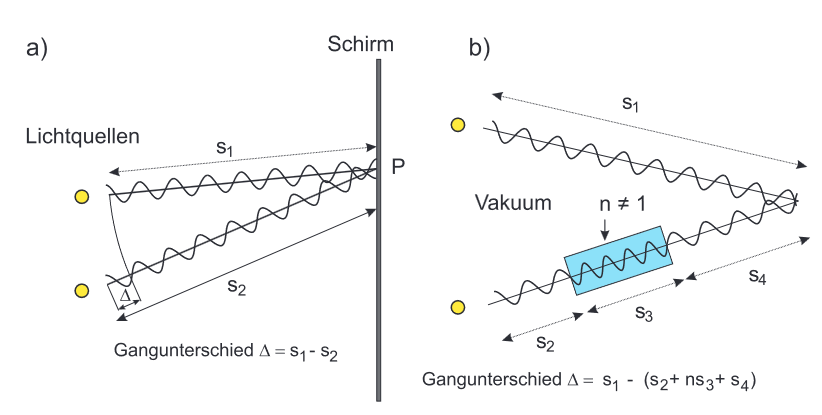
\includegraphics[width=0.9\textwidth]{graphics/skript/gangunterschiede.png}
    \caption{Gangunterschied bei: a) verschiedenen Weglängen; b) verschiedenen Medien [Quelle: PAP2.1 Skript, S.65, Stand: 22.03.2024]}
    \label{fig:gangunterschiede}
\end{figure}




\newpage
\subsubsection{Kohärenz}

Die Kohärenz einer Lichtquelle bedeutet, dass die Quelle Licht mit konstanter Phasenbeziehung aussendet, was eine weitere Voraussetzung für die Beobachtung von Interferenz darstellt. Ist Licht inkohärent, so sind die Phasenverschiebungen $\varphi$ statistisch verteilt. Dies ist beispielsweise bei den meisten Lichtquellen wie dem Sonnenlicht der Fall. Um also Interferenz zu beobachten ist es nötig, zunächst zwei kohärente Lichtstrahlen zu erzeugen, beispielsweise indem man eine Lichtquelle über eine Doppellochblende in zwei kohärente Wellenfronten aufteilt. 

Eine wichtige Eigenschaft ist die soganannte Kohärenzlänge $L$. Sie setzt sich zusammen aus der Kohärenzzeit $\tau$, dem Zeitraum, in dem ein Wellenzug mit konstanter Phasenbeziehgung von einer Quelle emittiert wird, sowie der Lichtgeschwindigkeit $c$:

\begin{equation}
    L = \tau c.
\end{equation}

Die Kohärenzlänge beschränkt also, wie groß der Gangunterschied zweier Lichtstrahler einer Quelle sein darf, da größere Unterschiede als $L$ dafür sorgen würden, dass die Strahlen nicht mehr aus dem selbem Emissionstakt stammen und somit nicht mehr interferieren. Bei Temperaturstrahlern ist diese Länge für gewöhnlich sehr klein, bei Lasern kann sie dafür aber bis zu viele Kilometer lang werden.


\subsubsection{Spektrale Bandbreite}

Da reale Lichtquellen nicht monochromatisch sind, enthalten sie immer Frequenzen innerhalb eines Intervalls $\omega_0 \pm \Delta \omega /2$, wobei $\Delta \omega$ die spektrale Bandbreite bezeichnet. Betrachten wir eine Lichtquelle mit rechteckigem Frequenzspektrum:

\begin{equation}
    g(\omega) =
    \begin{cases} 
    \vert g_0 , & |\omega - \omega_0| \leq \Delta \omega / 2 \\
    \vert 0 , & |\omega - \omega_0| > \Delta \omega / 2 \\
    \end{cases}
\end{equation}

Wir haben also eine Überlagerung aller auftretenden Frequenzen und erhalten nach einigen Umformungen:

\begin{equation}
    \begin{split}
        E_S &= \int_{-\infty}^\infty g(\omega) e^{i(\omega t - k z)} dw = \int_{-\Delta \omega / 2}^{\Delta \omega / 2} g_0 e^{i(\omega t - k z)} dw\\
        &= g_0 \Delta \omega \frac{\sin{\left(\Delta \omega / 2 (t - z/c) \right)}}{\Delta \omega / 2 (t - z/c)} e^{i\omega_0 (t - z/c)}
    \end{split}
\end{equation}

Diese Wellenform ist in Abbildung \ref{fig:spektrBandbreite} zu sehen. Man kann die Intensität des Wellenpakets aus dem Quadrat der Amplitude berechnen wobei sich zeigt, dass das erste Nebenmaximum nur etwa 4,7\% der Intensität des Hauptmaximums beträgt und die weiteren Nebenmaxima mit 1,7\%, 0,8\%, 0,5\% usw sehr schnell abfallen. Es steckt also nahezu die gesamte Intensität des Wellenpakets im Hauptmaximum und man kann eine endliche Breite des Wellenpakets annehmen, welche der Breite des Hauptmaximums von $4 \pi c / \Delta \omega$ entspricht. 
Wenn sich also zwei solche Wellen überlagern und dabei eine relative Verschiebung von $\Delta z = 2 \pi c / \Delta \omega$ aufweisen, so fällt das Maximum des einen auf die erste Nullstelle des anderen. Für solche Wellenpakete kann man also die Kohärenzlängee folgendermaßen annehmen:

\begin{equation}
    L = \frac{2 \pi c}{\Delta \omega}.
\end{equation}

Diese können wir auch über die Wellenlänge mit $\Delta \omega = 2 \pi \Delta \nu = 2 \pi c \Delta \lambda / \lambda^2$ ausdrücken:

\begin{equation}
    L = \frac{\lambda^2}{\Delta \lambda}.
\end{equation}


\begin{figure}[!b]
    \centering
    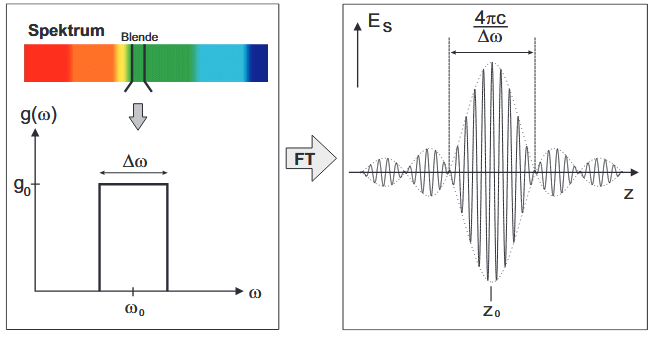
\includegraphics[width=0.7\textwidth]{graphics/skript/spektrale bandbreite.png}
    \caption{Rechteckförmiges Spektrum mit resultierender Wellenform [Quelle: PAP2.1 Skript, S.66, Stand: 24.03.2024]}
    \label{fig:spektrBandbreite}
\end{figure}



\clearpage
\newpage
\subsubsection{Interferenz gleicher Neigung}

Die Interferenz gleicher Neigung ist das Resultat, wenn ein Lichtbündel auf eine transparente, planparallele Platte trifft. Fällt dieses unter dem Winkel $\alpha$ auf die Platte der Dicke $d$ mit dem Brechungsindex $n$, so wird ein Teil reflektiert und der andere nach Snellius in der Platte gebrochen. Analog tritt beides auf, wenn der Lichtstrahl wieder von Innen den Plattenrand erreicht. Es gilt nun, dass alle Teilbündel interferieren, die im gleichen Neigungswinkel auf die Platte treffen. Dies lässt sich über den Gangunterschied $\Delta$ herleiten. Betrachten wir Abbildung \ref{fig:gleicheNeigung} so ergibt sich:

\begin{equation}
    \Delta = n ( \overline{AB} + \overline{BC} ) - \overline{AD} = \frac{2nd}{\cos{\beta}} - 2d \tan{\beta} \sin{\alpha}
\end{equation}

Mit dem Snellius'schen Brechungsgesetz erhalten wir:

\begin{equation}
    \begin{split}
        \Delta &= \frac{2nd}{\cos{\beta}} - \frac{2nd \sin^2{\beta}}{\cos{\beta}} \\
        &= 2nd \cos{\beta} \\
        &= 2d \sqrt{n^2 - \sin^2{\alpha}}.
    \end{split}
\end{equation}

Unter Berücksichtigung des Phasensprungs von $\pi$ bei der Reflexion an einem optisch Dichten Medium ergibt sich schlussendlich:

\begin{equation}
    \Delta = 2d \sqrt{n^2 - \sin^2{\alpha}} - \frac{\lambda}{2}.
\end{equation}

\begin{figure}[!b]
    \centering
    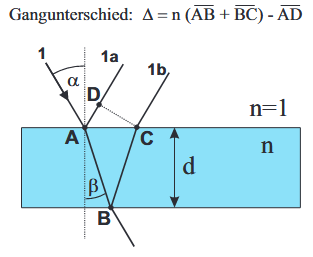
\includegraphics[width=0.4\textwidth]{graphics/skript/gleiche neigung.png}
    \caption{Interferenz gleicher Neigung [Quelle: PAP2.1 Skript, S.69, Stand: 24.03.2024]}
    \label{fig:gleicheNeigung}
\end{figure}

Wird nun eine Sammellinse in den Strahlengang eingebracht, so beobachtet man Interferenz der Teilbündel 1a, 1b, ... . Hier gilt nun die bereits erwähnte Regel, dass alle Bündel, die in gleichem Neigungswinkel einfallen miteinander im gleichen Punkt interferieren. In Abbildung \ref{fig:gleicheNeigung2} links ist ein zweidimensionaler Fall dargestellt, wo unterschiedliche Neigungswinkel zu unterschiedlichen Interferenzpunkten führen. Im Dreidimensionalen gilt dieselbe Regel, nur dass alle Bündel mit gleichem Neigungswinkel nun nicht in einem Punkt, sondern in einem Kreisring interferieren, wodurch sich das in Abbildung \ref{fig:gleicheNeigung2} rechts dargestellte Bild ergibt.

\phantom{.}

\begin{figure}[!h]
    \centering
    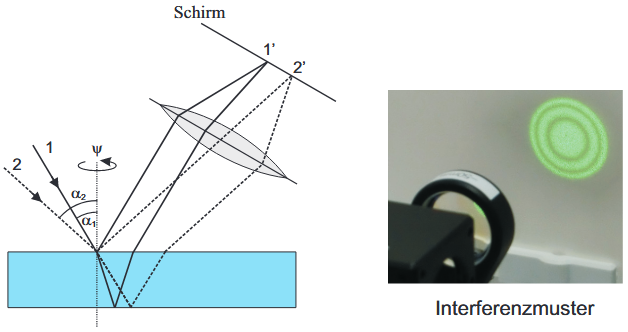
\includegraphics[width=0.9\textwidth]{graphics/skript/gleicheneigung2.png}
    \caption{Interferenz gleicher Neigung - 2D \& 3D [Quelle: PAP2.1 Skript, S.69, Stand: 24.03.2024]}
    \label{fig:gleicheNeigung2}
\end{figure}



\newpage
\subsubsection{Interferenz gleicher Dicke}

Die Interferenz gleicher Dicke ist das Phänomen, wenn paralleles Licht auf eine keilförmige Platte trifft und  die Bündel interferieren, die auf einem Streifen parallel zur Keilkante, ergo für die $d(x) = $ konst. gilt, einen gleichen Gangunterschied haben und so ein streifenförmiges Interferenzmuster bilden. Anhand von Abbildung \ref{fig:gleicheDicke} lässt sich der Gangunterschied für kleine Keilwinkel $\epsilon$ herleiten als:

\begin{equation}
    \Delta \approx 2 \ d(x) \ \sqrt{n^2 - \sin^2{\alpha}} - \frac{\lambda}{2}.
\end{equation}

Fällt zudem das Licht fast senkrecht auf den Keil ($\sin{\alpha} \approx 0$), so ergibt sich:

\begin{equation}
    \Delta \approx 2 \ d(x) \ n - \frac{\lambda}{2}.
\end{equation}

Somit ändert sich der Gangunterschied $\Delta$ mit der Keildicke $d(x)$ und man stellt die genannten Interferenzbedingungen fest.

\phantom{.}

\begin{figure}[!h]
    \centering
    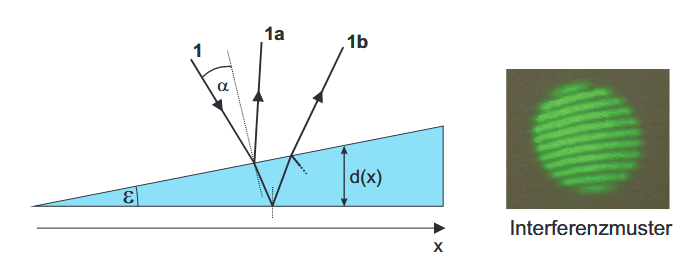
\includegraphics[width=0.9\textwidth]{graphics/skript/gleiche dicke.png}
    \caption{Interferenz gleicher Dicke [Quelle: PAP2.1 Skript, S.69, Stand: 24.03.2024]}
    \label{fig:gleicheDicke}
\end{figure}


\newpage
\subsubsection{Das Michelson-Interferometer}

Grundsätzlich besteht das Michelsoninterferometer aus einer Lichtquelle deren Strahl auf einen Strahlteiler trifft, wodurch zwei Strahlengänge erzeugt werden, die eine Hälfte des Strahls trifft auf einen kipparen und die andere auf einen verschiebbaren Spiegel, wo diese reflektiert werden und danach beide über den Strahlenteiler zu einem Schrim beziehungsweise Detektor zur Analyse geleitet werden, zu sehen in Abbildung \ref{fig:Michelsoninterferometer}a. Wir bezeichnen den Kippwinkel des einen Spiegels mit $\epsilon$ und die verschobene Strecke des anderen mit $\Delta x$. Sind beide Spiegel parallel, so tritt Interferenz gleicher Neigung auf und der Gangunterschied beträgt in Richtung des Winkels $\alpha$

\begin{equation}
    \Delta = 2 \Delta x \cos{\alpha} - \frac{\lambda}{2}.
\end{equation}

\begin{figure}[!b]
    \centering
    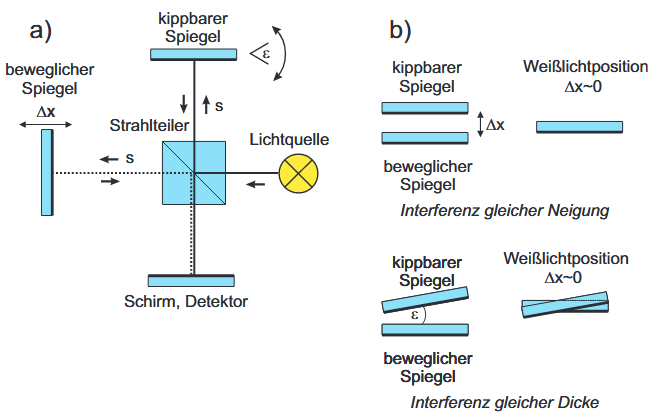
\includegraphics[width=0.8\textwidth]{graphics/skript/interferometer.png}
    \caption{Michelsoninterferometer [Quelle: PAP2.1 Skript, S.70, Stand: 24.03.2024]}
    \label{fig:Michelsoninterferometer}
\end{figure}

Hier wurde $n=1$ angenommen und man beobachtet das erwartete Ringsystem. Betrachten wir das Zentrum, ergo $\alpha = 0$, so gilt für $\Delta x = \lambda / 2$ auch $\Delta = \lambda / 2$ und das Minimum 0-ter Ordnung liegt im Zentrum. Bei $\Delta x = 3\lambda / 4$ beträgt der Gangunterschied $\lambda$ und das Maximum 1. Ordnung liegt im Zentrum bei konstanter Verschiebung werden also nacheinander verschiedenen Interferenzordnungen im Zentrum durchlaufen.  \\
Neigt man den anderen Spiegel, so tritt Interferenz gleicher Dicke auf. Diese kann sich auch mit der Interferenz gleicher Neigung überlappen, wenn gleichzeitig der Spiegel verschoben wird. 

\newpage
Man kann mithilfe dieser Prinzipien die Wellenlänge der verwendeten Lichtquelle bestimmen. Misst man, wie weit man den Spiegel verschiebt $\Delta x$ und wieviele Interferenzstreifen dabei vorbeilaufen $\Delta m$, so ergibt sich die Wellenlänge als

\begin{equation}
    \lambda = 2 \frac{\Delta x}{\Delta m}.
    \label{eq:1_WELLENLÄNGE_A1}
\end{equation}

Auch kann man den Brechungsindex von Luft bestimmen, indem man in einen Interferometerschenkel eine Glasküvette einbringt, deren innerer Luftdruck variiert werden kann, was den Brechungsindex $\Delta n$ und somit die optische Weglänge verändert. Dabei laufen wieder $\Delta m$ Intrerferenzstreifen auf einem Schirm vorbei. Hat die Küvette dabei eine Länge von $a$ so ergibt sich:

\begin{equation}
    \begin{split}
        \Delta &= 2 a \Delta n, \\
        \Rightarrow \Delta m &= \frac{\Delta}{\lambda} = 2a \frac{\Delta n}{\lambda}, \\
        \Rightarrow \Delta n &= \frac{\lambda}{2a} \Delta m.
    \end{split}
\end{equation}

Variiert man den Druck über den gesamten verfügbaren Bereich von Vakuum bis Luftdruck $b$ so gilt $\Delta n = n(\text{Luft}) - n(\text{Vakuum}) =  n - 1 $ und wir erhalten:

\begin{equation}
    n(\lambda, T, b) - 1 = \frac{\lambda}{2a} \Delta m(b).
\end{equation}

Daraus kann man den Brechunsindex $n_0$ bei Normalbedinungen, ergo $T_0 = 273,15$K \& $p_0 = 101325$Pa, berechnen, indem man den Luftdruck $p$ sowie die Raumtemperatur $T$ zur Zeit des Versuchs aufnimmt:

\begin{equation}
    (n_0 - 1) = (n - 1) \frac{p_0 T}{p T_0} = \frac{\lambda p_0 T}{2 a T_0} \frac{\Delta m}{p}.
    \label{eq:1_BRECHUNGSINDEX_A2}
\end{equation}

Zuletzt kann man mit dem Interferometer auch die Kohärenzlänge von Lichtquellen untersuchen, wenn der Gangunterschied der beiden Arme nicht größer als die Kohärenzlänge ist. Für die dann auftretende ''Weißlichtinterferenz'' müssen die Arme nahezu gleich lang sein, wenn eine Leuchtdiode mit sehr kleiner Kohärenzlänge beobachtet wird. Die Position bezeichnet man dann als Weißlichtposition. Beobachtet man das Interferenzbild mit einem Oszilloskop, so kann man, wenn man den Spiegel durch die Weißlichtposition fahren lässt, eine Momentaufnahme von Signal machen, das aus dem kurzen Moment resultierte, wo die Weißlichtposition getroffen wurde. Das Oszilloskop zeichnet hierbei die Zeit $t$ auf, in der sich der Spiegel genau in dieser Position befand, aus der man mit der Verfahrgeschwindigkeit des Spiegels $v$ die Länge bestimmen kann, die die Spiegelarme maximal auseinander liegen dürfen, damit noch Interferenz entsteht. Nimmt man diese Strecke mal 2 für den Hin- und Rückweg des Lichts so erhält man die Kohärenzlänge $L$ der Lichtquelle:

\begin{equation}
    L = 2 v t
    \label{eq:1_Kohärenzlänge_A3}
\end{equation}


\newpage
\subsection{Versuchsaufbau}

Das von uns verwendete Interferometer ist in Abbildung \ref{fig:Aufbau} zu sehen. Der Grundaufbau ist das normale bereits beschriebene Michelsoninterferometer mit Lichtquelle, Strahlteiler, Spiegeln und Schrim beziehungsweise Detektor zur Analyse. Als Lichtquellen stehen ein Laser und eine Leuchtdiode zur Verfügung. An den Spiegeln sind Schrauben angebracht, mit denen diese vertikal und horizontal gekippt werden können. Es stehen mehrere Schirme zur Verfügung, mit denen in der Position vor dem Detektor das Bild analysiert oder in den Positionen 1 \& 3 Strahlengänge ausgeblendet werden können, sowie eine Glasküvette mit Vakuumpumpe und Manometer die in Position 3 in den Strahlengang eingebracht werden kann. 
Der Spiegel bei Position 1 lässt sich mechanisch sowohl manuell mit einem Regler als auch um eine feste Strecke vor oder zurück per Knopfdruck verstellen, wobei die Position von einer Messuhr gemessen wird. 

Zusätzlich stehen ein Oszilloskop und ein Diskriminator zur Verfügung. Ersteres zeichnet die Signale des Detektors auf und Letzterer dient dazu, die Maxima beim Verschieben des Spiegels zu zählen. Dazu verstärkt dieser das Signal des Oszilloskops und wandelt es in Rechtecksignale um. Die Empfindlichkeit kann hierbei auch reguliert werden, sodass die ideale Einstellung gefunden werden kann. 


\begin{figure}[!b]
    \centering
    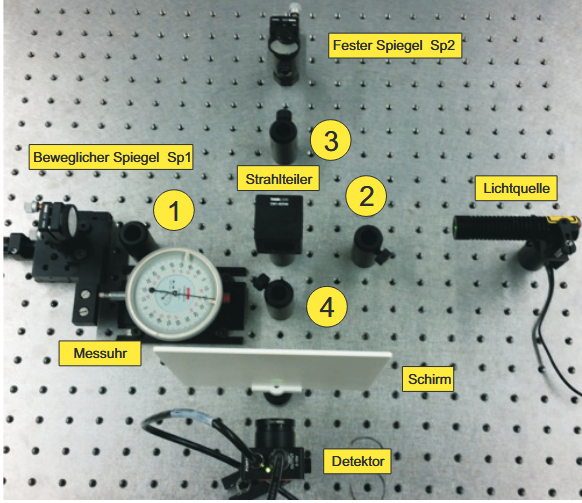
\includegraphics[width=0.7\textwidth]{graphics/skript/aufbau.png}
    \caption{Versuchsaufbau [Quelle: PAP2.1 Skript, S.72, Stand: 24.03.2024]}
    \label{fig:Aufbau}
\end{figure}


%---------------VERSUCHSPROTOKOLL MIT MESSDATEN---------------
\newpage

\section{Versuchsprotokoll mit Messdaten}

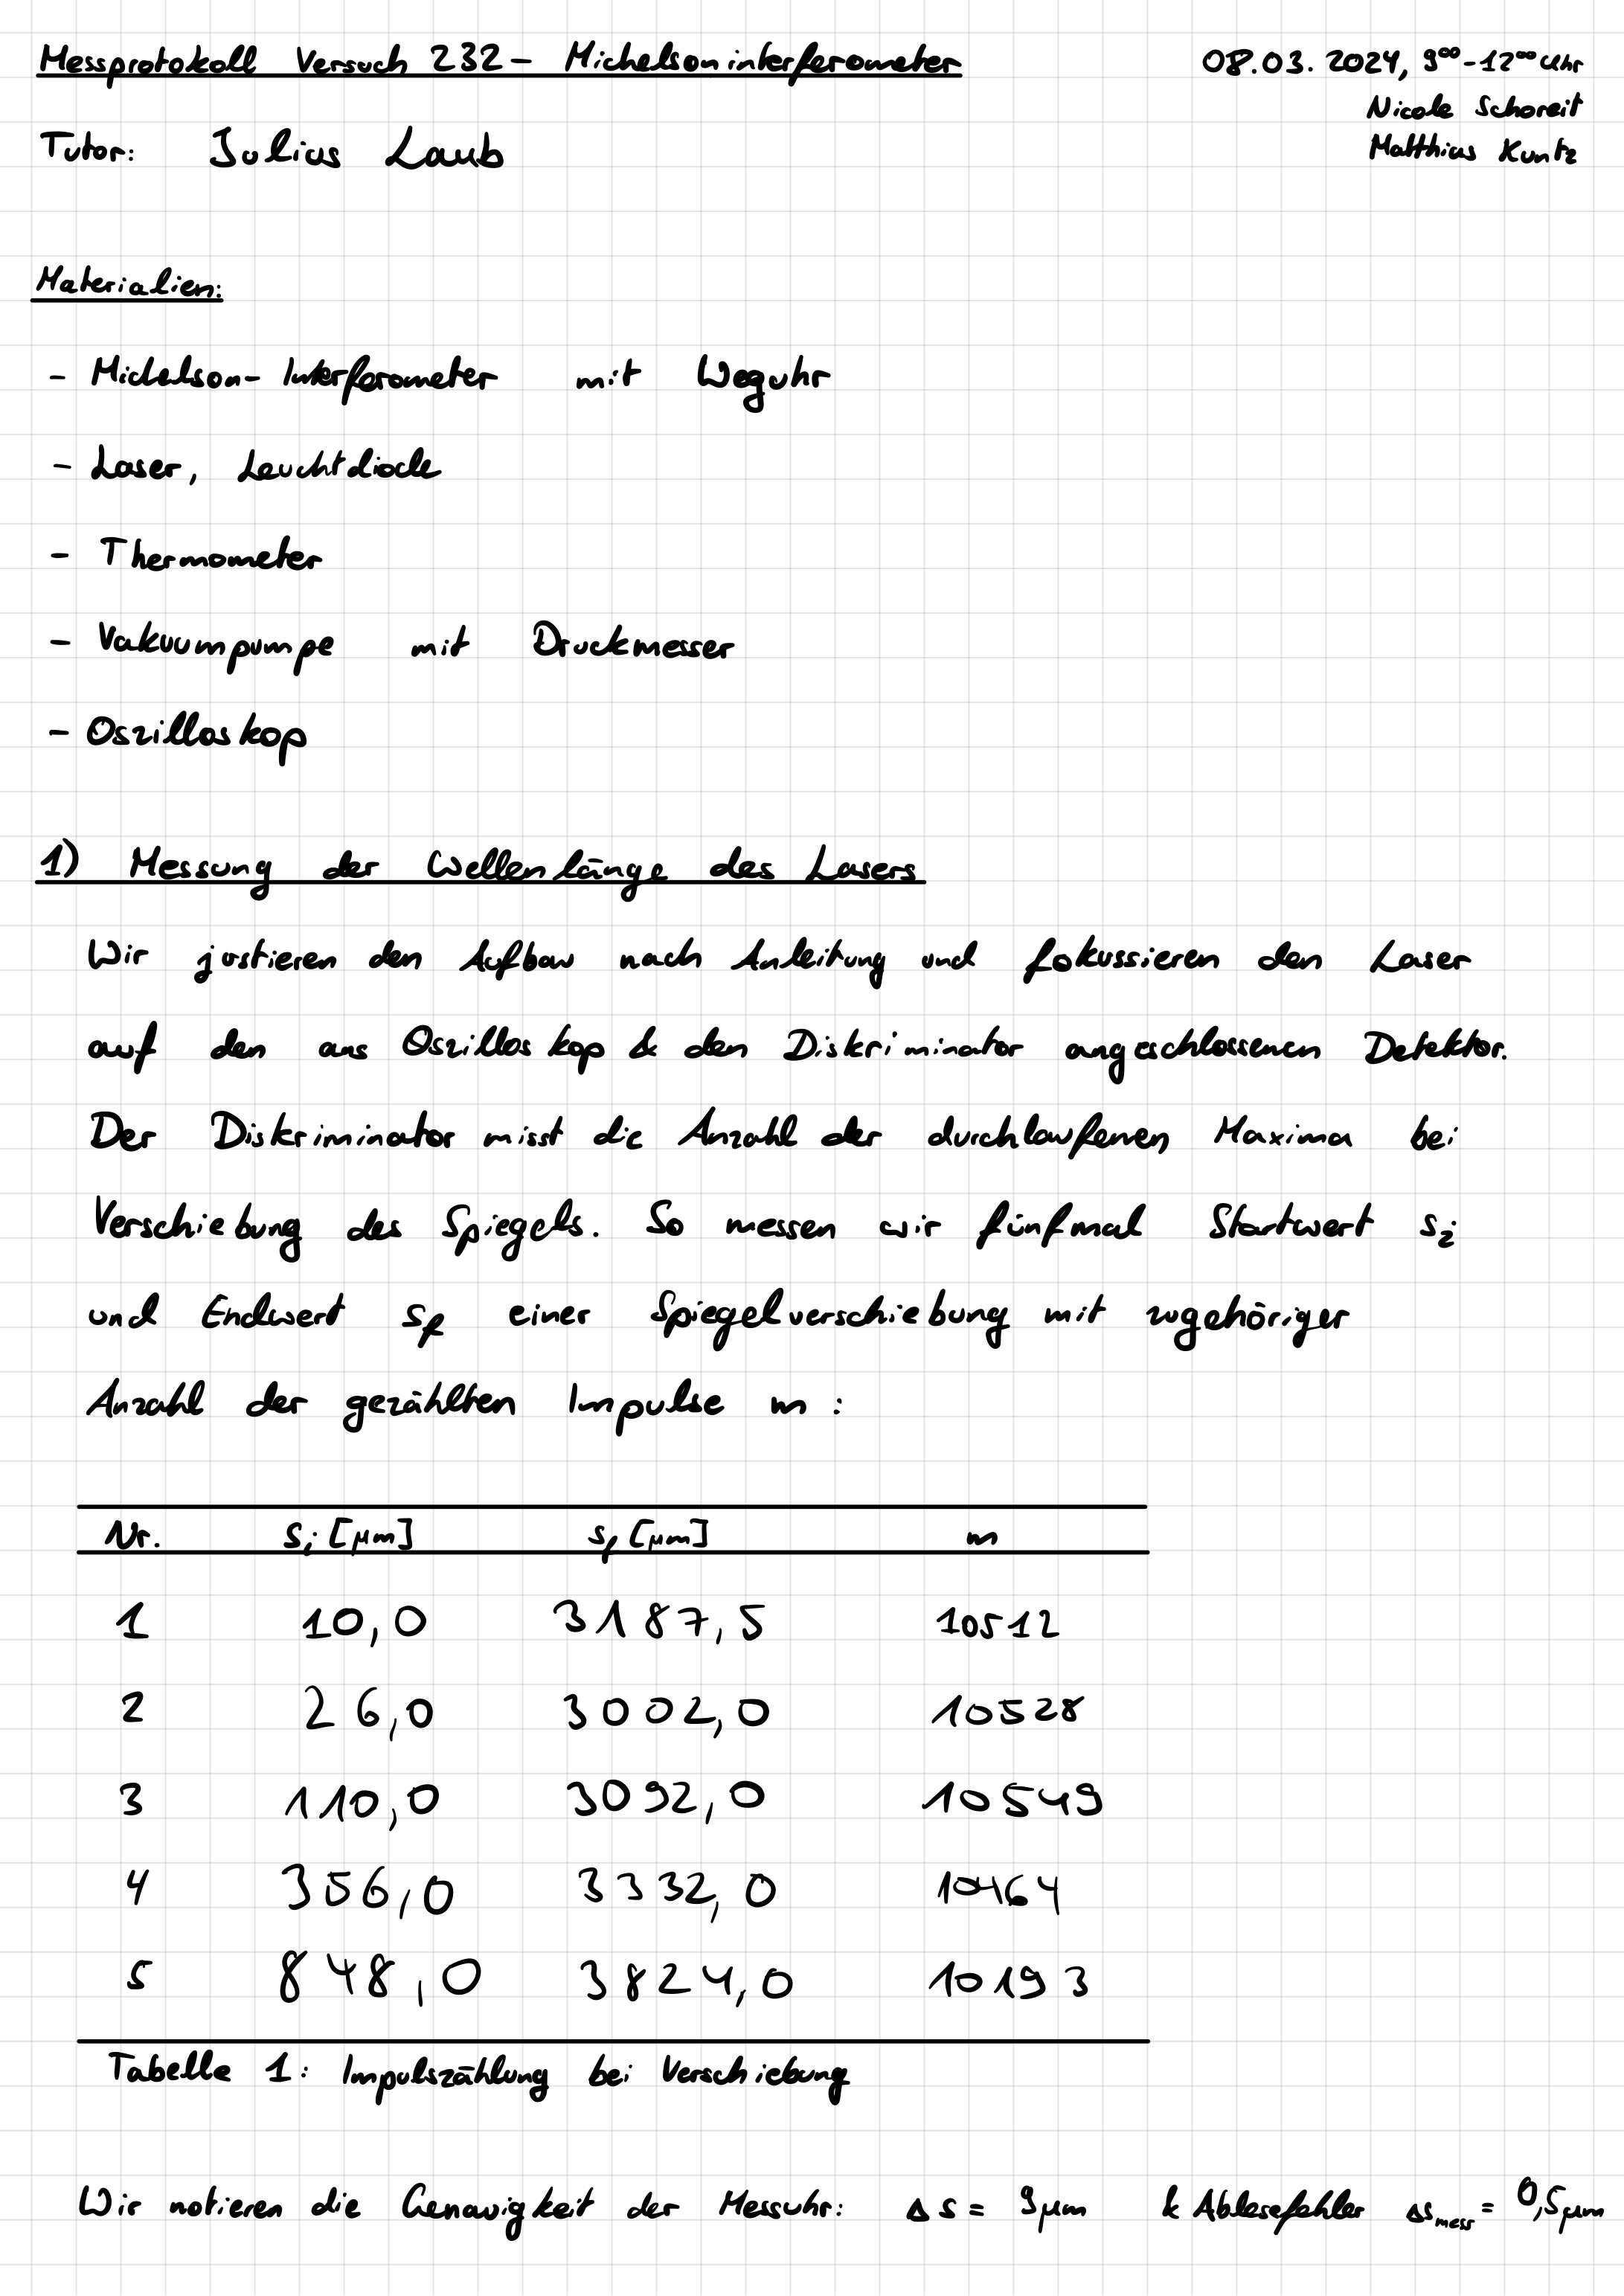
\includegraphics[width=\textwidth]{graphics/mess1.jpg}
\newpage
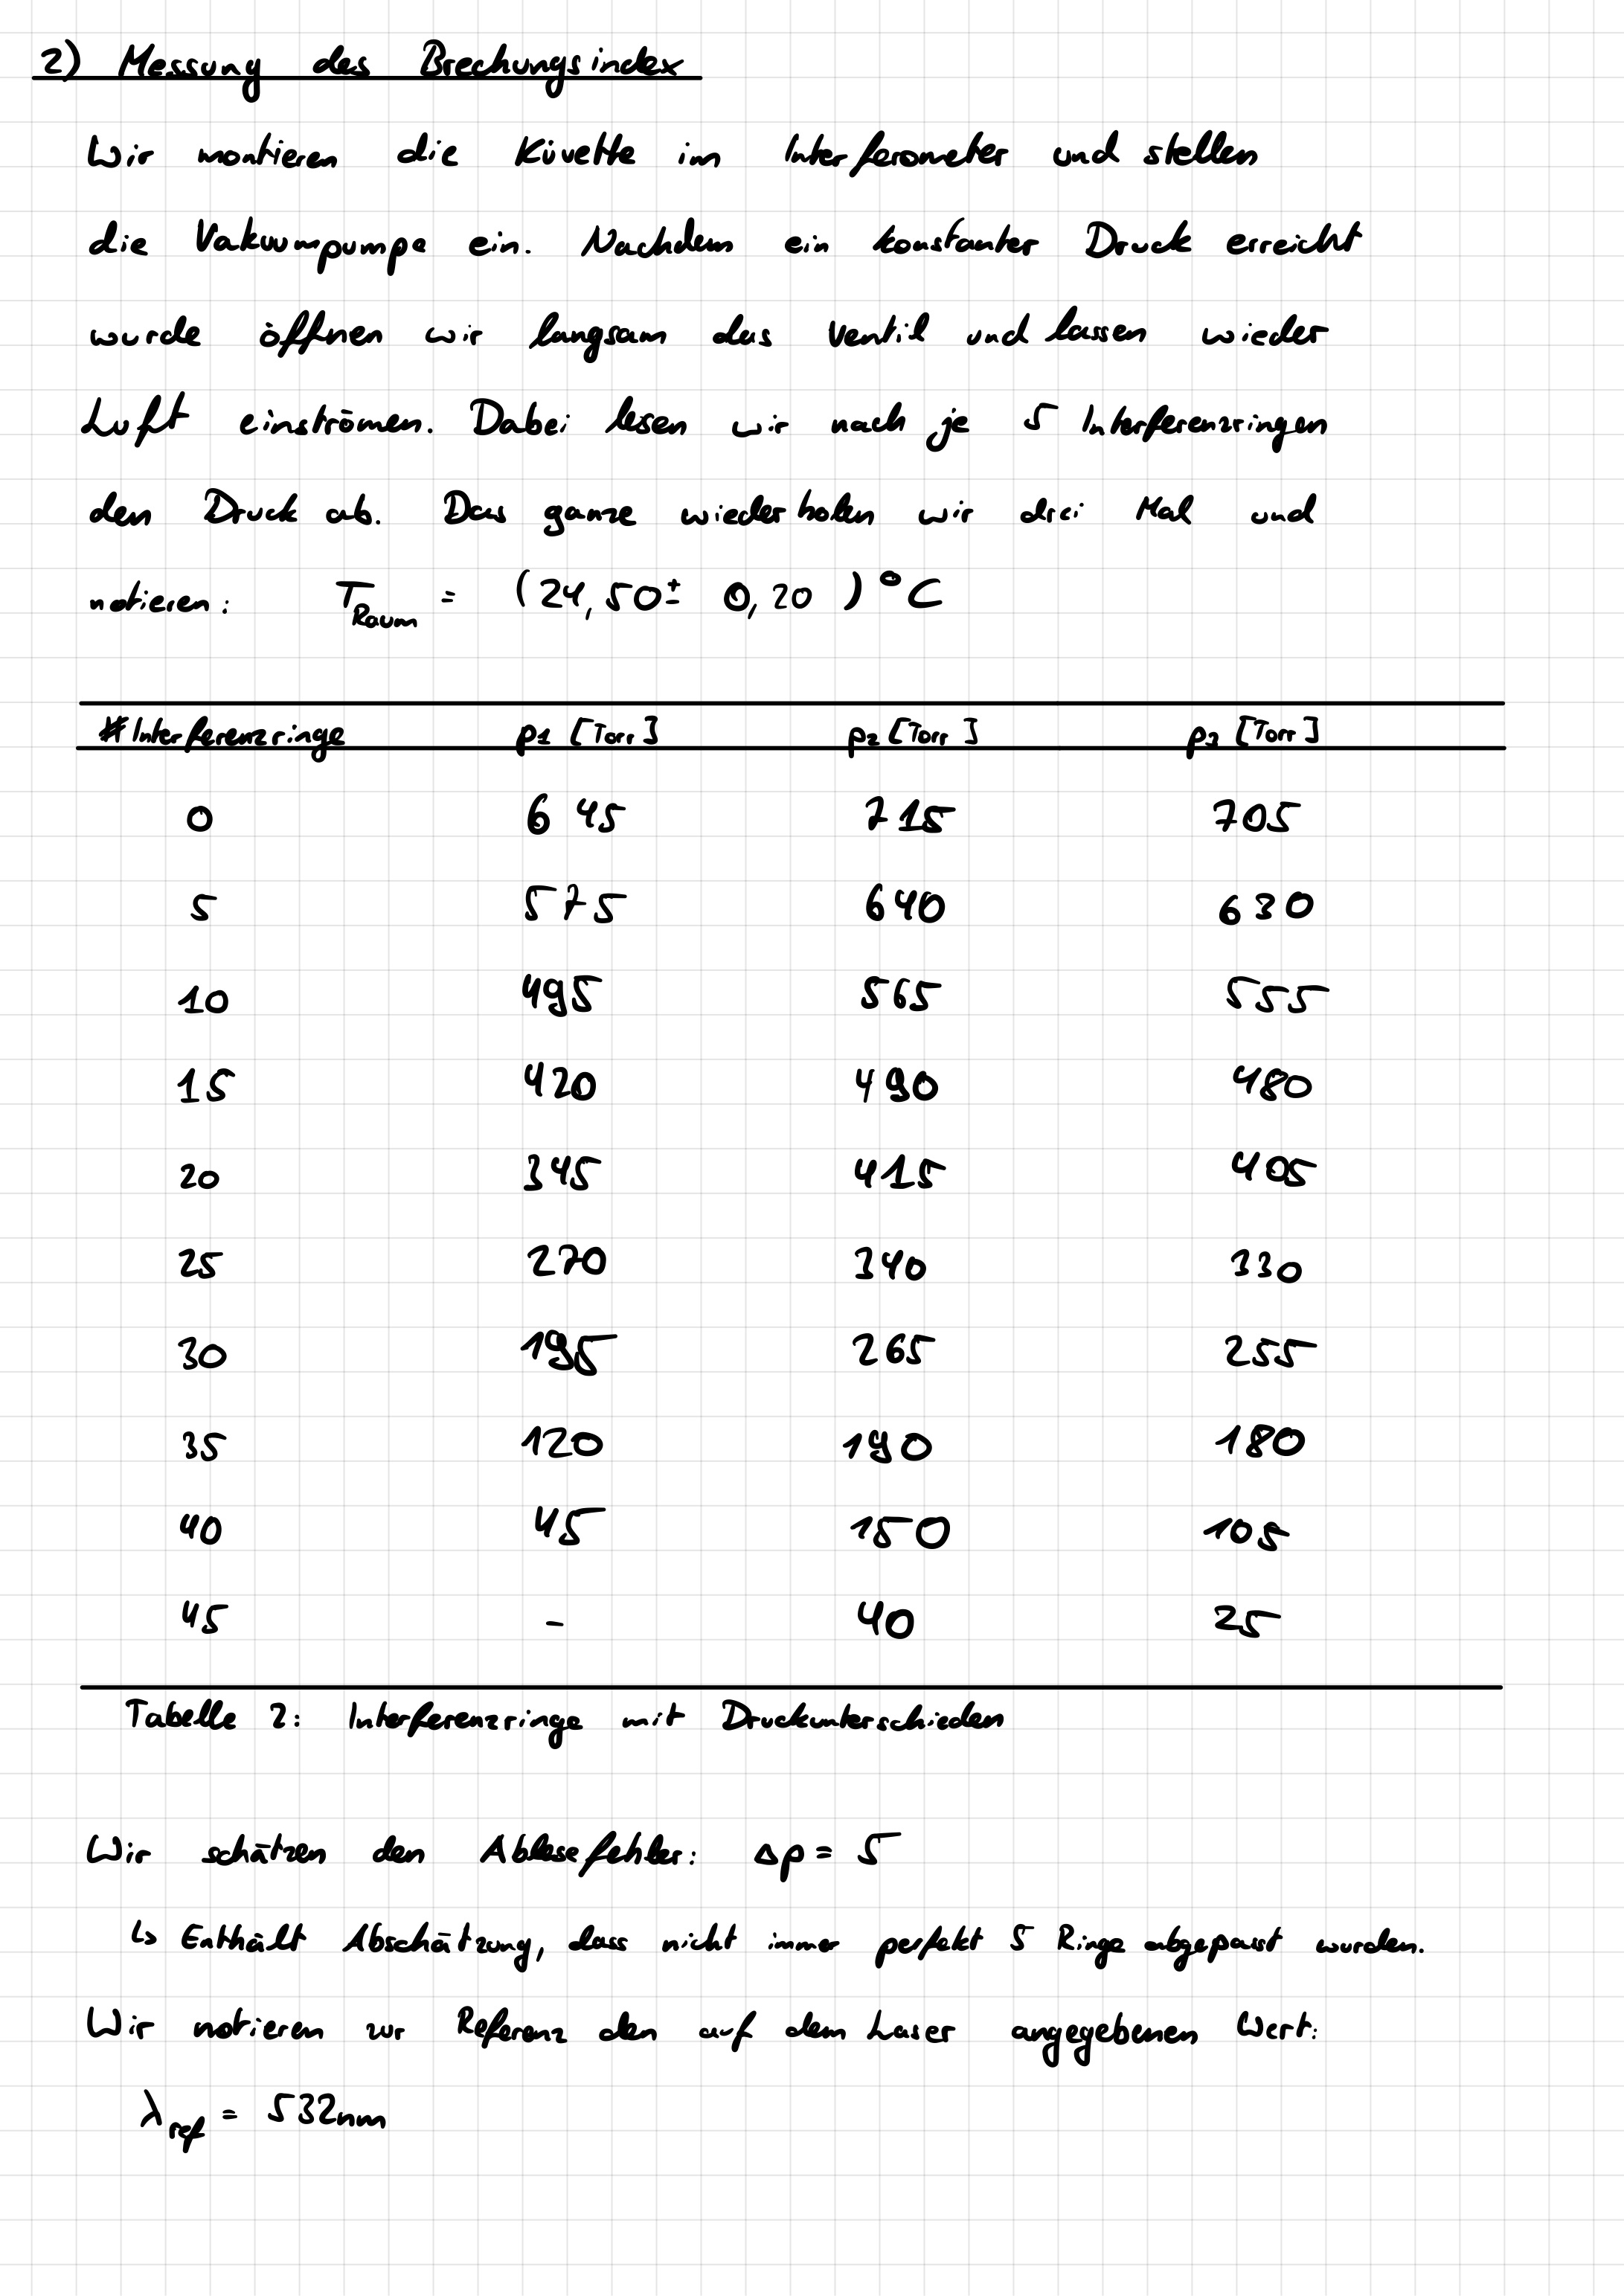
\includegraphics[width=\textwidth]{graphics/mess2.jpg}
\newpage
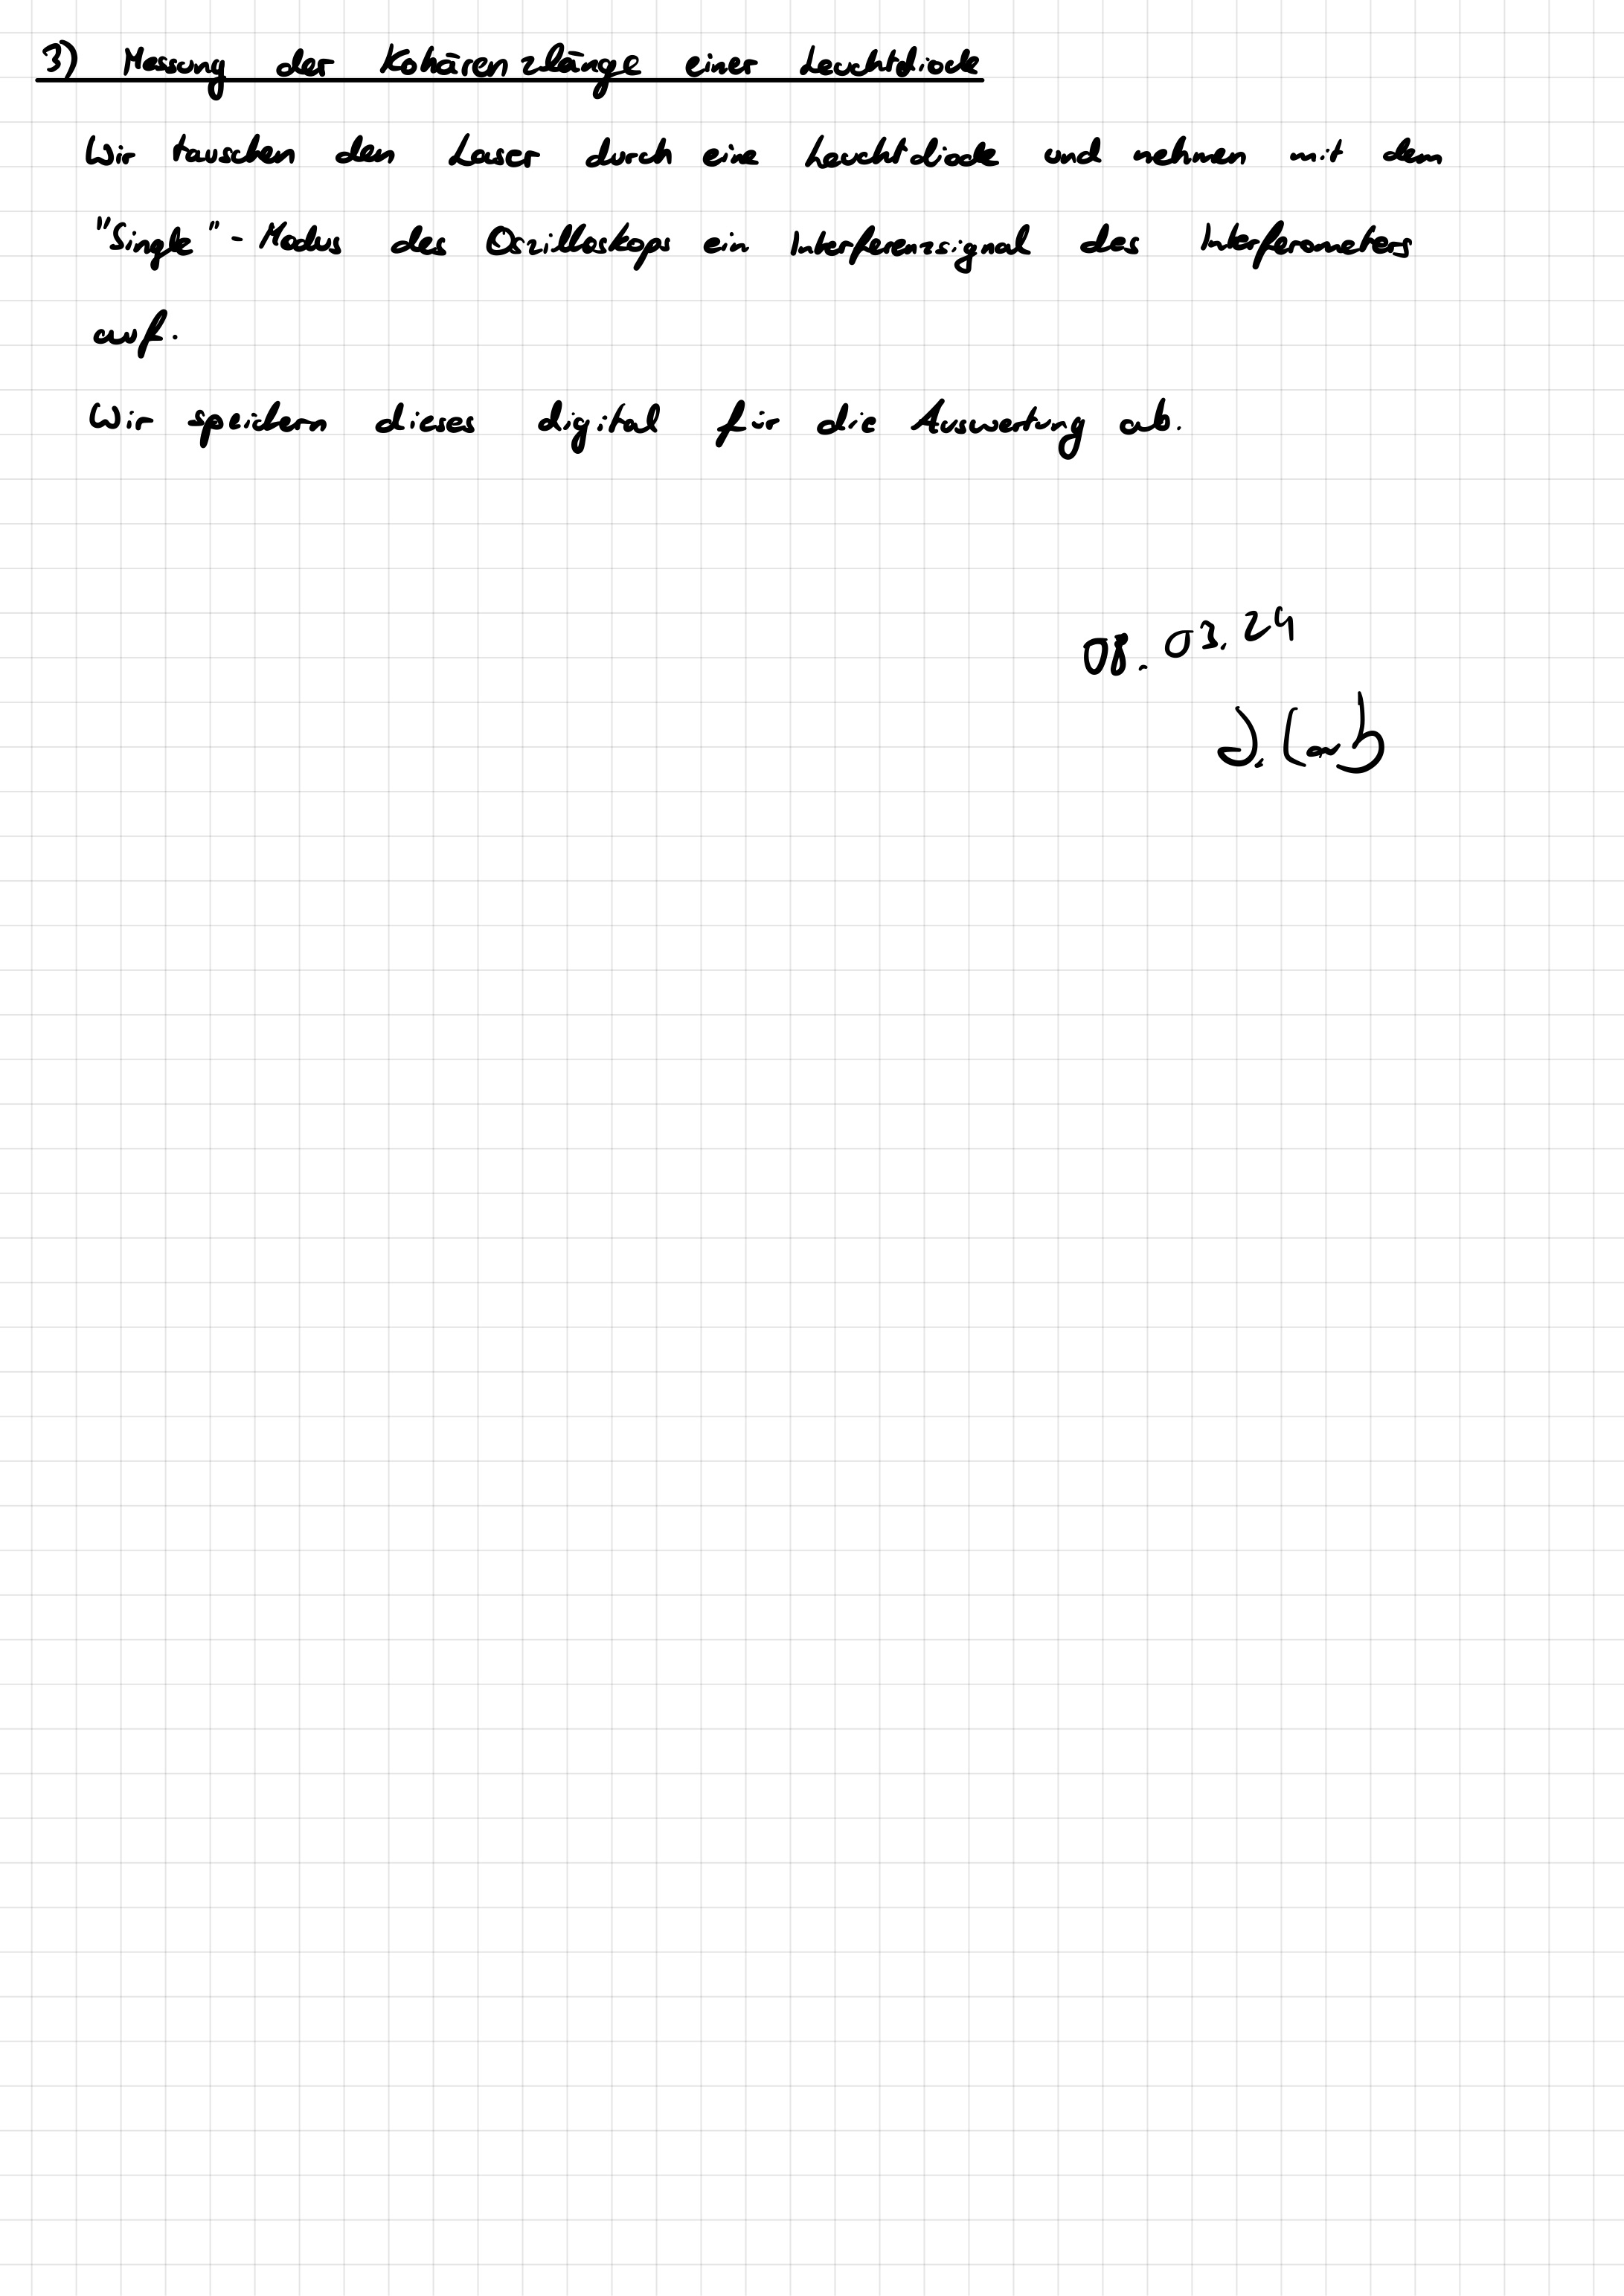
\includegraphics[width=\textwidth]{graphics/mess3.jpg}
\newpage

\addtocounter{table}{2}

\newpage
%-------------------------AUSWERTUNG-------------------------
\section{Auswertung}

In dieser Evaluation werden alle Fehler, sofern keine spezifische Angabe gemacht wird, mithilfe der Gauss'schen Fehlerfortpflanzung berechnet. Dies bedeutet, dass ein Wert $F$, der mit der Formel $f(a_1, ..., a_n)$ berechnet wird, den Fehler $\Delta F$ annimmt:

\begin{equation}
    \Delta F = \sqrt{\sum_n \left( \frac{\partial f}{\partial a_n} \cdot \Delta a_n \right)^2}.
\end{equation}

Des Weiteren erfolgen Signifikanztests von zwei Werten $a$ und $a'$ über die folgende Formel:

\begin{equation}
    \sigma = \frac{|a-a'|}{\sqrt{(\Delta a)^2 + (\Delta a')^2}}.
\end{equation}

Die Auswertung sowie Berechnung erfolgen über das dem Dokument angehängte Python-Programm.

\newpage

\subsection{Die Wellenlänge des grünen Lasers}

Wir beginnen, indem wir mit den Messungen von Versuchsteil 1 die Wellenlänge des grünen Lasers bestimmen. Hier haben wir den Spiegel immer eine bestimmte Strecke verschoben wobei wir Start- und Endposition sowie die Anzahl der durchlaufenen Maxima fünf Mal gemessen haben. Aus den gemessenen Start- und Endwerten $s_i$ \& $s_f$ berechnen wir zunächst die Differenz $\Delta s = s_f - s_i$. Der Fehler ergibt sich dabei, da unser angegebener Ablesefehler von 0,5$\mu$m keine signifikanten Einfluss hätte, rein aus der systematischen Ablesegenauigkeit der Messuhr von $\Delta (\Delta s) = 9 \mu$m bei dem von uns verwendeten 3mm Messbereich. 

Anschließend berechnen wir nach Gleichung \ref{eq:1_WELLENLÄNGE_A1} die Wellenlängen für jede Messung. Der Fehler berechnet sich dabei mit:

\begin{equation}
    \Delta \lambda = \frac{2}{m} \cdot \Delta (\Delta s).
\end{equation}

Somit erhalten wir die in Tabelle \ref{tab:5LAMBDAS} eingetragenen Ergebnisse.

\phantom{.}

\begin{table}[!h]
    \centering
    %\resizebox{\textwidth}{!}{
    \begin{tabular}{cccc}
        \hline
        \textbf{Nr} & $\bm{m}$ & $\bm{\Delta s}$ [$\mu$m] & $\bm{\lambda}$ [nm]  \\ \hline
             1 & 10512 & 3177 $\pm$ 9 & 604,5 $\pm$ 1,7 \\
             2 & 10528 & 2976 $\pm$ 9 & 565,3 $\pm$ 1,7 \\
             3 & 10549 & 2982 $\pm$ 9 & 565,4 $\pm$ 1,7 \\
             4 & 10464 & 2976 $\pm$ 9 & 568,8 $\pm$ 1,7 \\
             5 & 10193 & 2976 $\pm$ 9 & 583,9 $\pm$ 1,8 \\ \hline
    \end{tabular}%}
    \caption{Berechnung der Wellenlänge $\lambda$ für jede Messreihe}
    \label{tab:5LAMBDAS}
\end{table}

\phantom{.}

Aus den berechneten fünf Wellenlängen kann man nun den Mittelwert $\overline{\lambda}$ berechnen. Der Fehler ergibt sich dabei aus dem Standardfehler des Mittelwerts $\sigma_{std}$ sowie den Fehlern der einzelnen $\lambda$'s:

\begin{equation}
    \begin{split}
        \Delta \overline{\lambda} &= \sqrt{\sigma_{std}^2 + \left( \frac{1}{N} \sum_{i=1}^N \Delta \lambda_i \right)^2} \\
        \text{mit} \ \ \ \sigma_{std} &= \sqrt{\frac{1}{N(N-1)} \sum_{i=1}^N (\overline{\lambda} - \lambda_i)^2}.
    \end{split}
    \label{eq:FEHLER_MW}
\end{equation}

Somit erhalten wir als Ergebnis für die Wellenlänge des grünen Lasers:

\begin{equation}
    \bm{\overline{\lambda} = (578 \pm 8)} \textbf{nm}.
\end{equation}

Zum Vergleich dieses Wertes verwenden wir die Herstellerangabe des Lasers von $\lambda = (532 \pm 1)$nm und machen einen Signifikanztest. Es ergibt sich eine Abweichung von $\sigma_\lambda = 5,83$. Dies liegt außerhalb der $3\sigma$-Umgebung und ist somit eine signifikante Abweichung. Es muss also irgendein grundlegender systematischer Fehler vorgelegen haben, was vor allem daran zu sehen ist, dass alle unsere berechneten Wellenlängen in Tabelle \ref{tab:5LAMBDAS} zu groß sind. Grund könnte beispielsweise eine systematische Ungenauigkeit des Diskriminators beim Zählen der Maxima sein.


\newpage
\subsection{Der Brechungsindex von Luft}

Wir verwenden unsere Messungen des Luftdrucks in der im Strahlengang eingebrachten Küvette um den Brechungsindex von Luft $n_0$ zu bestimmen. Nach Gleichung \ref{eq:1_BRECHUNGSINDEX_A2} ergibt sich dieser nämlich aus der Steigung einer Geraden von $\Delta m$ über dem Druck $p$. Für unsere gemessenen Druckwerte berücksichitgen wir noch den Fehler der Güteklasse 0,6, indem wir als Fehler unserer Druckwerte $\Delta p = 5$Torr annehmen.

Nun plotten wir unsere Messwerte des Drucks für alle drei Messreihen separat als Funktion der durchlaufenen Interferenzringe. Der Grund dafür ist, dass so von der gleich verwendeten Fit-Funktion des 'Scipy'-Package die y-Fehler der Druckwerte berücksichtigt werden. So können wir nun jeweils eine lineare Funktion an die Messwerte fitten und aus dem Kehrwert der Steigung $\alpha$ somit drei Werte von $s = \Delta m / p$ berechnen, deren Mittelwert dann den Endwert gibt. Die drei Diagramme mit Fitgeraden sind in Abbildung \ref{fig:PLOTs_DRUCK_INTERFERENZRINGE} zu sehen und die Ergebnisse der Fitparameter in Tabelle \ref{tab:STEIGUNGEN}. Dabei verwenden wir:

\begin{equation}
    \begin{split}
        s &= \frac{\Delta m}{p} = \frac{1}{\alpha}, \\
        \Rightarrow \Delta s &= s \frac{\Delta \alpha}{\alpha}
    \end{split}
\end{equation}

\phantom{.}

\begin{table}[!h]
    \centering
    %\resizebox{\textwidth}{!}{
    \begin{tabular}{ccc}
        \hline
        \textbf{Nr.} & $\bm{\alpha}$ [Torr] & $\bm{s}$ [1/Torr] \\ \hline
             1 & -15,05  $\pm$ 0,04 & -0,06645 $\pm$ 0,00019 \\
             2 & -14,70  $\pm$ 0,24 & -0,0680 $\pm$ 0,0011  \\
             3 & -15,05  $\pm$ 0,03 & -0,06643 $\pm$ 0,00014 \\ \hline
    \end{tabular}%}
    \caption{Steigungen und Verhältnis $s = \Delta m/p$}
    \label{tab:STEIGUNGEN}
\end{table}

\phantom{.}

Für den Mittelwert erhalten wir nun unter Verwendung derselben Fehlerformel wie in Gleichung \ref{eq:FEHLER_MW}:

\begin{equation}
    \overline{s} = (67,0 \pm 0,7) \cdot 10^{-3} \frac{1}{\text{Torr}}
\end{equation}

Somit können wir nun Gleichung \ref{eq:1_BRECHUNGSINDEX_A2} verwenden und den Brechungsindex von Luft bei Normalbedingungen $n_0$ berechnen. Dazu benötigen wir noch die Temperatur und Druck unter Normalbedingungen $T_0 = 273,15$K \& $p_0 = 101325 \text{Pa} = 760$Torr, das Innenmaß der Küvette $a = (50,00 \pm 0,05)$mm sowie die in unserem Messprotokoll verzeichnete Raumtemperatur $T = (297,7 \pm 0,2)$K. Für die Wellenlänge des Lasers verwenden wir aufgrund der hohen Abweichung im ersten Teil die Herstellerangabe $\lambda = (532 \pm 1)$nm. Somit erhalten wir:

\begin{equation}
    \begin{split}
        n_0 &= \frac{\lambda}{2a} s \frac{p_0 T}{T_0} + 1 \\
        \Rightarrow \Delta n_0 &= n_0 \sqrt{\left( \frac{\Delta \lambda}{\lambda} \right)^2 + \left( \frac{\Delta a}{a} \right)^2 + \left( \frac{\Delta s}{s} \right)^2 + \left( \frac{\Delta T}{T} \right)^2} \\ \\
        &\Rightarrow \bm{n_0 = 1,000 \ 295 \pm 0,000 \ 003} 
    \end{split}
\end{equation}

Wir vergleichen diesen Wert über einen Signifikanztest mit dem Litearturwert $n_{0,lit} = 1,00028$ und erhalten eine Abweichung von $\sigma_{n_0} = 4,72$. Diese Abweichung ist außerhalb der $3\sigma$-Umgebung und somit signigfikant. Grund hierfür könnten ein unterschätzter Fehler des Manometers oder eine überschätzte Genauigkeit des Vorgangs, genau 10 Interferenzringe zu durchlaufen, sein. Auch können Unterschiede in Luftfeuchtigkeit, Raumtemperatur und Luftdruck im Raum für Abweichungen vom Literaturwert gesorgt haben.

\begin{figure}[!bp]
  \centering
  \subfloat[Messreihe 1]{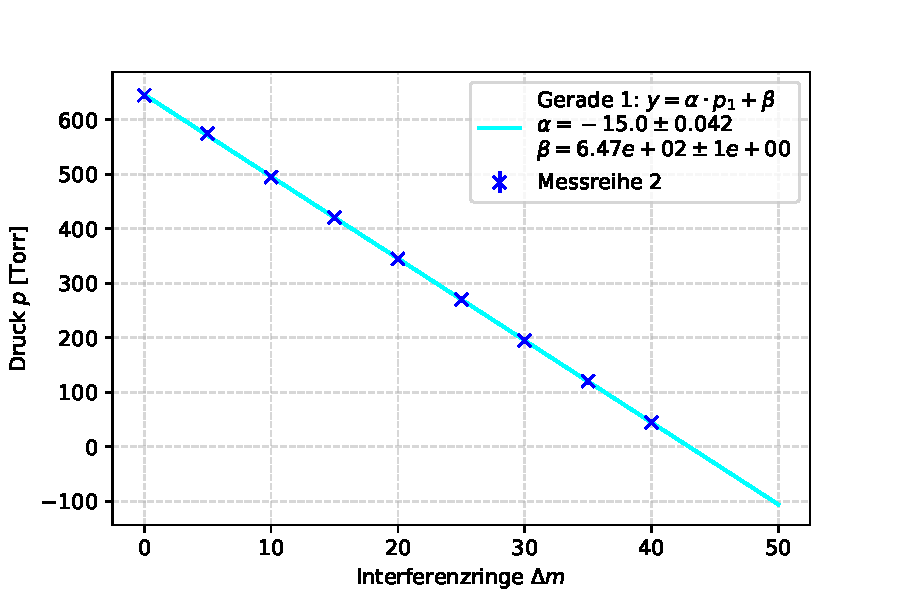
\includegraphics[width=0.65\textwidth]{graphics/plots/Brechungsindex1.pdf}}
  \hfill
  \subfloat[Messreihe 2]{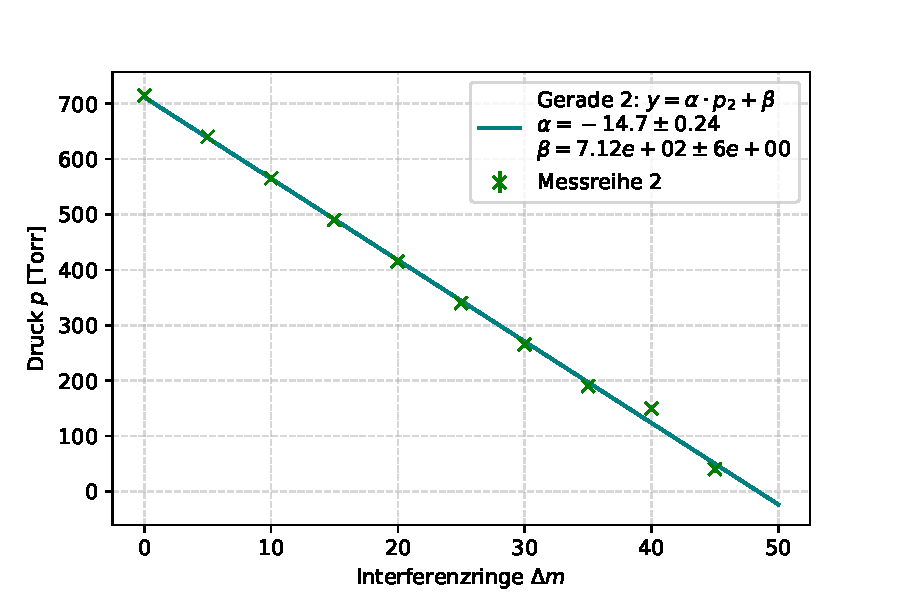
\includegraphics[width=0.65\textwidth]{graphics/plots/Brechungsindex2.pdf}}
  \hfill
  \subfloat[Messreihe 3]{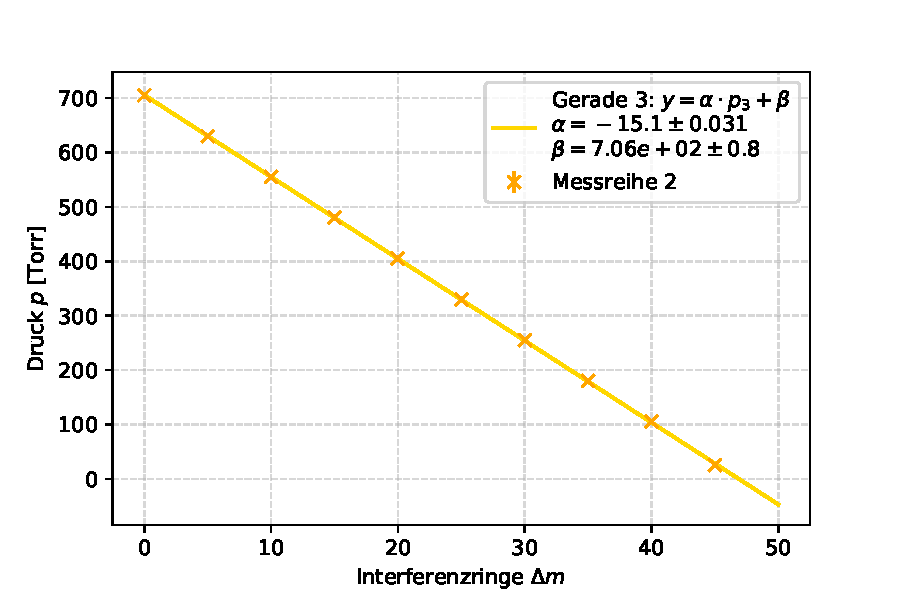
\includegraphics[width=0.65\textwidth]{graphics/plots/Brechungsindex3.pdf}}
  \hfill
  \caption{Plots des Drucks gegen die durchlaufenen Interferenzringe}
  \label{fig:PLOTs_DRUCK_INTERFERENZRINGE}
\end{figure}



\newpage
\subsection{Die Kohärenzlänge der Leuchtdiode}

Aus dem digital aufgezeichneten Signal von Teil Drei möchten wir nun die Kohärenzlänge der verwendeten Leuchtdiode berechnen. Dazu gehen wir wie folgt vor:

Zunächst importieren wir das abgespeicherte Signal in Python. Daraufhin verwenden wir das ''Scipy''-Package, um uns die Peaks der Funktion berechnen zu lassen. Beides ist zu sehen in Abbildung \ref{fig:KohärenzlängeMessung}a \& b. Nun verwenden wir die soeben bestimmten Peaks und fitten eine Gaußfunktion an diese an, um die einhüllende Welle zu erhalten. Der Gaußfit, zu sehen in Abbildung \ref{fig:KohärenzlängeMessung}c, berechnet die folgenden Fit-Parameter:

\begin{equation}
    \begin{split}
        G(t; \mu, \sigma) &= \frac{a}{\sqrt{2 \pi} \sigma} \exp{\left( -\frac{(t - \mu)^2}{2 \sigma^2} \right)} \\
        a &= -(1135 \pm 17) \cdot 10^{-6} \\
        \mu &= (13,4 \pm 0,3) \cdot 10^{-3} \text{s} \\
        \sigma &= -(14,4 \pm 0,3) \cdot 10^{-3} \text{s} \\
    \end{split}
\end{equation}

Aus der Standardabweichung $\sigma$ können wir die Halbwertsbreite $t_\frac{1}{2}$ der Gaußfunktion berechnen, welche benötigt wird um die Kohärenzlänge abzuschätzen. Da unser Fitwert der Standardabweichung negativ ist, nehmen wir einfach den Betrag für die Berechnung, da uns nur der absolute Wert interessiert. Die Halbwertsbreite berechnet sich allgemeingültig nach:

\begin{equation}
    \begin{split}
        t_\frac{1}{2} &= 2 \sqrt{2 \ln{(2)}} \sigma \\
        \Rightarrow \Delta t_\frac{1}{2} &= 2 \sqrt{2 \ln{(2)}} \cdot \Delta \sigma \\ \\
        &\Rightarrow t_\frac{1}{2} = (0,0338 \pm 0,0006) \text{s}
    \end{split}
\end{equation}

Nun können wir mithilfe von Gleichung \ref{eq:1_Kohärenzlänge_A3} die Kohärenzlänge $L$ abschätzen, wobei wir für $v$ die maximale Verfahrgeschwindigkeit des Motors von $v = 0,1$mm/s verwenden:

\begin{equation}
    \begin{split}
        L &= 2 v t_\frac{1}{2} \\
        \Rightarrow \Delta L &= 2 v \cdot \Delta t_\frac{1}{2} \\ \\
        &\Rightarrow \bm{L = (6,76 \pm 0,12) \cdot 10^{-6}} \textbf{m}.
    \end{split}
\end{equation}

Zwar haben wir für diesen Wert keinen Literaturwert, man kann ihn aber qualtitativ bewerten und feststellen, dass er die Theorie nicht verletzt. Die Kohärenzlänge der Leuchtdiode ist wie erwartet sehr kurz und liegt im Mikrometer-Bereich, somit erscheint der Wert durchaus sinnvoll.

\begin{figure}[!bp]
  \centering
  \subfloat[Aufnahme des Oszilloskops]{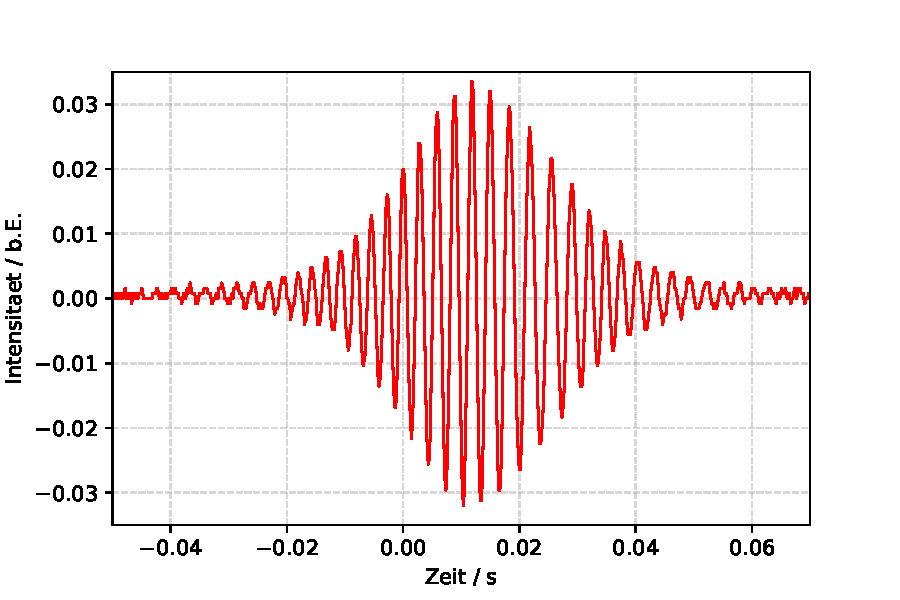
\includegraphics[width=0.48\textwidth]{graphics/plots/interferogramm_raw.pdf}}
  \hfill
  \subfloat[Bestimmung der Peaks]{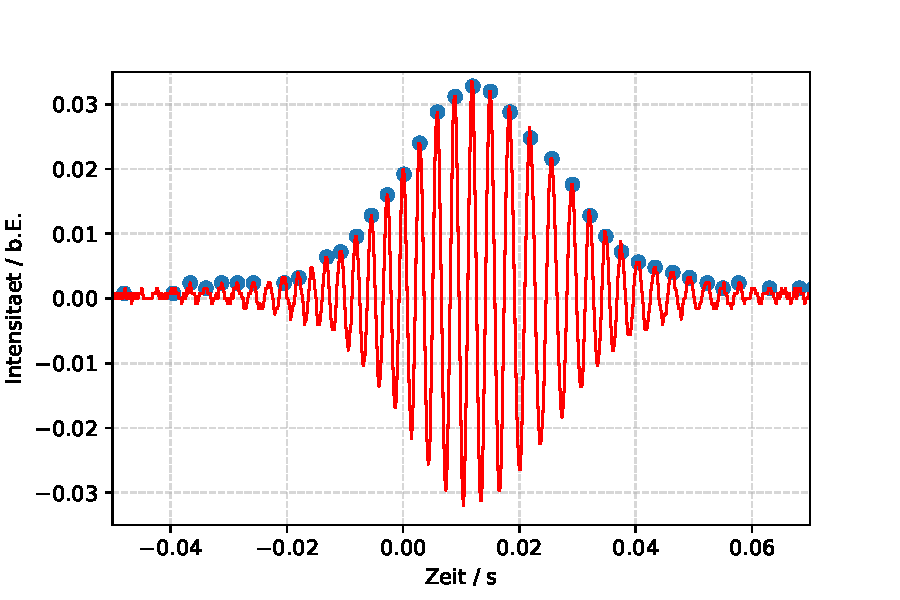
\includegraphics[width=0.48\textwidth]{graphics/plots/interferogramm_peaks.pdf}}
  \hfill
  \subfloat[Gaußfit]{\includegraphics[width=0.9\textwidth]{graphics/plots/interferogramm_gauß.pdf}}
  \hfill
  \caption{Interferogramm der Leuchtdiode}
  \label{fig:KohärenzlängeMessung}
\end{figure}

\clearpage
\newpage
%---------------PRÄSENTATION DER ENDERGEBNISSE---------------
\section{Zusammenfassung der Endergebnisse}

In diesem Versuch wurde mithilfe des Michelsoninterferometers die Wellenlänge eines Lasers, der Brechungsindex von Luft und die Kohärenzlänge einer Leuchtdiode bestimmt.

Zunächst beobachteten wir, wie viele Interferenzmaxima durchlaufen werden, wenn einer der beiden Spiegel der Interferometerarme um eine bestimmte Strecke verfahren wird. Aus diesen Messreihen errechneten wir die Wellenlänge des Lasers als 

\begin{equation}
    \lambda = (578 \pm 8) \text{nm}.
\end{equation}

Im Vergleich mit dem Literaturwert $\lambda = (532 \pm 1)$nm ergab sich hier eine signifikante Abweichung von $\sigma_\lambda = 5,83$. Dies lies auf einen systematischen Fehler schließen, da bei allen Messreihen stets zu große Werte für die Wellenlänge resultierten.

Anschließend berechneten wir den breechungsindex von Luft, indem wir eine Glasküvette mit Vakuumpumpe und Manometer in einen Interferometerarm einbrachten und bei Veränderung des Drucks die durchlaufenen Interferenzringe in konstanten Intervallen beobachteten. Wir bekamen hier das Ergebnis

\begin{equation}
    n_0 = 1,000 \ 295 \pm 0,000 \ 003.
\end{equation}

Erneut lieferte der Vergleich mit dem Literaturwert $n_{0,lit} = 1,00028$ eine signifikante Abweichung von $\sigma_{n_0} = 4,72$. Als Ursache wurden hier die Ungenauigkeit des Verfahrens sowie mögliche Schwankungen in Raumtemperatur, Luftdruck und Luftfeuchtigkeit genannt.

Zuletzt berechneten wir aus dem aufgenommenen Interferogramm des Oszilloskops die Kohärenzlänge der Leuchtdiode. Hier kamen wir auf 

\begin{equation}
    L = (6,76 \pm 0,12) \cdot 10^{-6} \text{m}.
\end{equation}

Da es keinen direkten Vergleichswert gab, ließ sich nur das Fazit ziehen, dass dieser Wert im Kontext der Theorie sinnvoll erscheint, da er wie erwartet sehr klein ist. 



\newpage
%---------------ZUSAMMENFASSUNG UND DISKUSSION---------------
\section{Diskussion}

Die Ergebnisse dieses Versuchs waren leider nicht ganz so passend wie gehofft. Zwar landeten alle Ergebnisse mit Vergleichswert immer in der Richtigen Größenordnung und waren auch, wie beispielsweise der Brechungsindex, ziemlich nah am Literaturwert, jedoch wiesen beide signifikante Abweichungen auf.

Im ersten Versuchsteil deutet alles wie bereits erwähnt auf einen systematischen Fehler. Alle fünf Messungen lieferten deutlich zu große Ergebnisse. Wenn wirklich ein solcher Fehler vorliegt würde das bedeuten, dass entweder die Strecken systematisch zu groß oder die Anzahl der Maxima systematisch zu klein gemessen wurde. Woran genau es jetzt liegt ist für uns im Nachhinein schwer zu sagen, dennoch würden wir eher auf einen Fehler beim Zählen des Diskriminators schließen. Beim Einstellen der Empfindlichkeit wurde diese nämlich so runtergedreht, dass keine Maxima gezählt werden, wenn sich der Spiegel nicht bewegt. Anfangs zählte dieser nämlich teils einfach von alleine hoch, ohne dass er eigentlich etwas detektieren sollte. Es ist durchaus möglich, dass er hierbei etwas zu weit runtergedreht wurde und deshalb einige Maxima nicht mitzählte, was eine Erklärung für die zu großen Wellenlängen sein könnte. Dies ist aber wie gesagt nur eine Vermutung und muss so keines Falls richtig sein. Im Kontext hiervon wird aber vermutlich die größte Fehlerquelle dieses Versuchsteils durchaus die Zählung des Diskriminators sein. Wie man diesen Aspekt aber verbessern könnte, ohne dass der Rahmen des Physikalischen Anfängerpraktikums gesprengt wird, ist auch nicht leicht zu sagen. Automatische oder genauere Justierungen des Diskriminators würden aber sicherlich bessere Ergebnisse liefern.

Der Zweite Versuchsteil wird seine größten Schwachstellen höchstwahrscheinlich in der Messung des Drucks in der Glasküvette mit dem Manometer und dem manuellen Abpassen von genau 10 Interferenzringen haben. Ersteres war nämlich durchaus häufig inkosistent, bis zu dem Punkt dass schon kleinere äußere Einflüsse bei geschlossenem Ventil dennoch die Anzeige veränderten. Letzteres war auch nicht gerade besser, da das exakte Öffnen und Schließen des Ventils und das Abpassen vom Zeitpunkt, in dem das Interferenzbild genauso aussieht wie im Schritt vorher durchaus mühsam waren. Hier hätten digitale Hilfen wie das Oszilloskop genutzt werden können, um genauer auf die 10 Ringe zu kommen. 

Im letzten Versuchsteil lässt sich aufgrund des fehlenden Referenzwerts nicht genau bewerten, was hätte verbessert werden können. Jedoch lässt sich sagen, dass die verwendete Vorgehensweise dem Zweck genügt, zu zeigen, dass die Kohärenzlänge einer Leuchtdiode wie erwartet sehr gering ist. Das fing schon während des Versuchs an indem schnell klar wurde, wie schwierig es ist die Weißlichtposition manuell zu finden. Somit rechtfertigt dies auch die recht ausführliche Justierung des Aufbaus und des Oszilloskops, die zur Beobachtung hier nötig ist. Wirklich viel Verbessern lässt sich hier also nicht wirklich, da das zu beobachtende Phänomen schon beim Versuch sehr deutlich gemacht und am Ende durch ein passendes Ergebnis bestätigt wurde.

Zusammenfassend lässt sich also sagen, dass zwar nicht immer exakte, aber durchaus zufriedenstellende Ergebnisse erzielt wurden. Die erhöhten Sigmaabweichung halten sich noch bedingt in Grenzen und zeigen somit, dass die Ergebnisse in der richtigen Umgebung landeten und nur an vereinzelten Stellen von Fehlern zurückgehalten wurden. 

\newpage
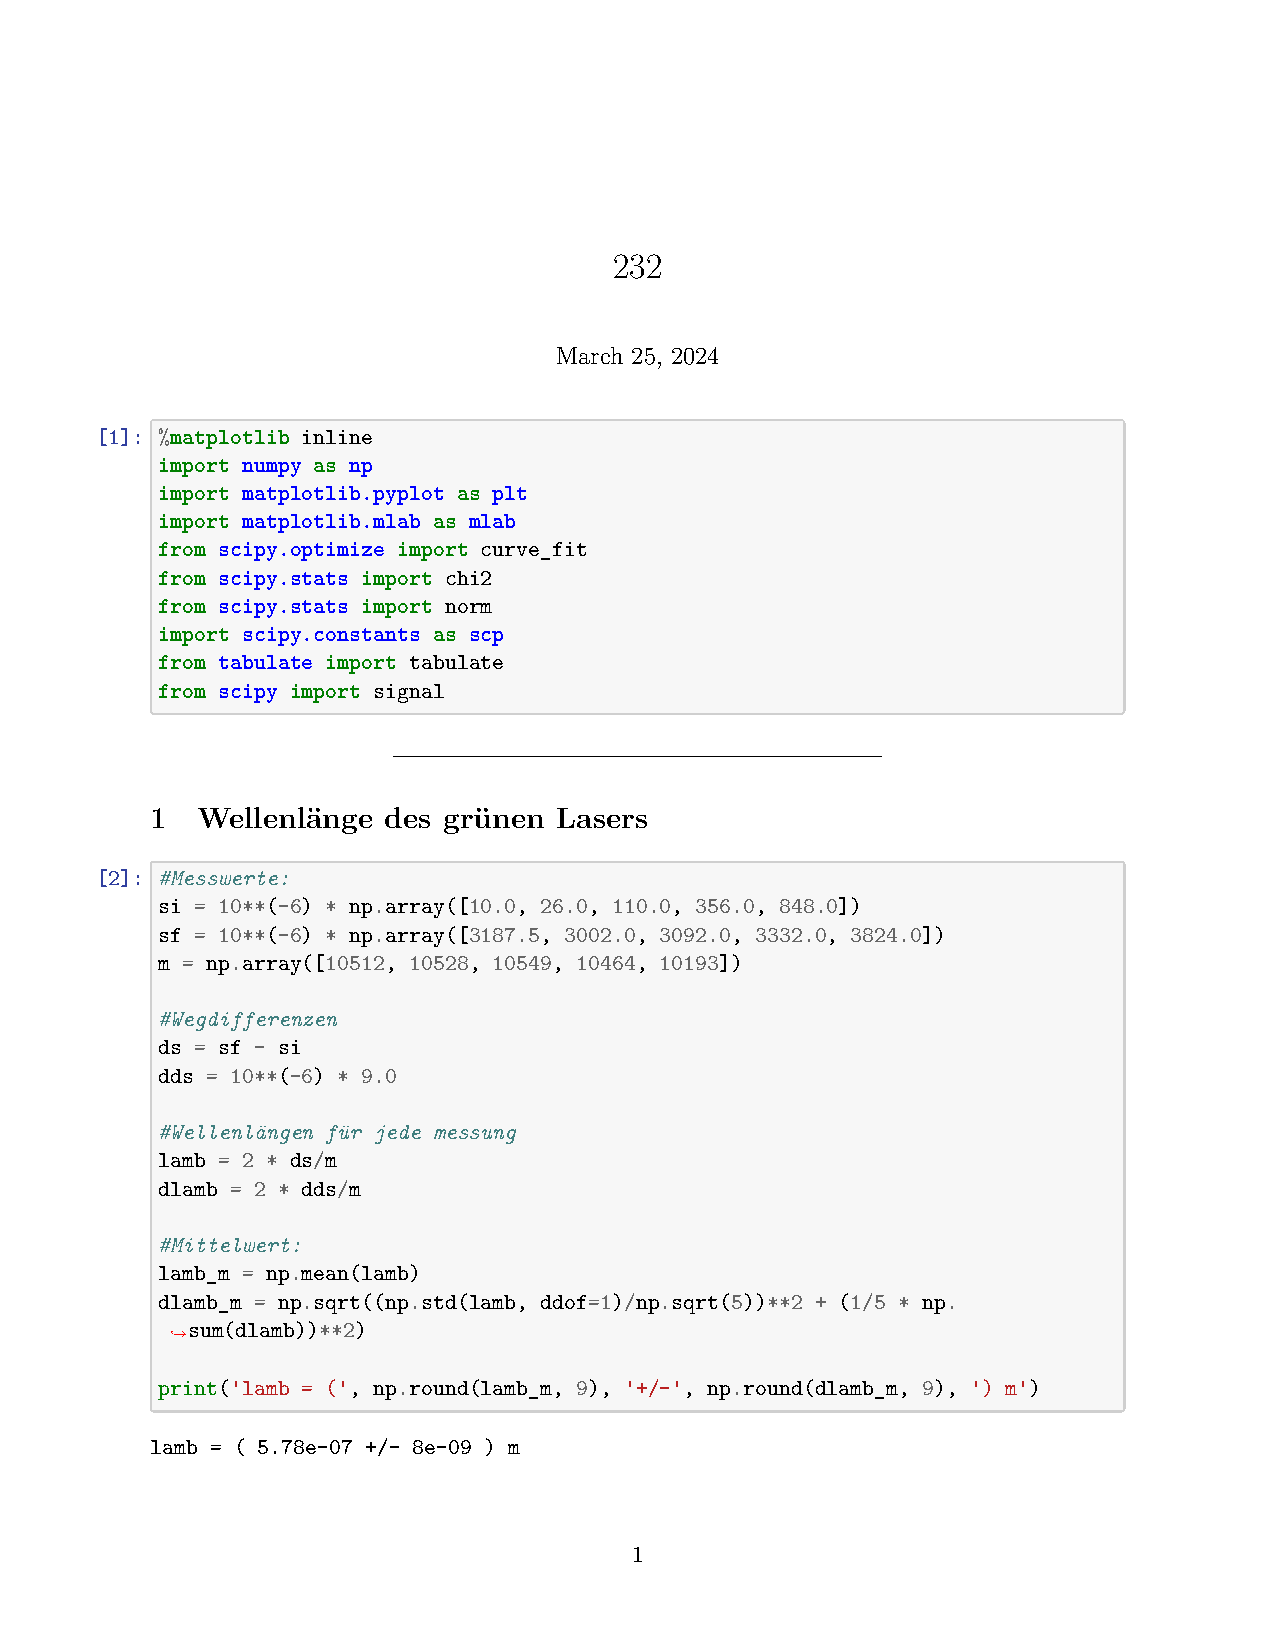
\includepdf[pages=-]{232.pdf}

\end{document}

